\documentclass[12pt]{article}
\usepackage[paperwidth=841mm,paperheight=1189mm,left=9mm,right=9mm,top=8mm,bottom=8mm]{geometry}
\usepackage[T1]{fontenc}\usepackage[utf8]{inputenc}\usepackage{lmodern}
\usepackage{graphicx,booktabs,tabularx,array,xcolor,enumitem,microtype,ragged2e,tikz}
\usetikzlibrary{arrows.meta,positioning}
\usepackage{tcolorbox}\tcbuselibrary{skins,breakable}
\pagestyle{empty}\setlength{\parindent}{0pt}\setlength{\parskip}{0.08em}
\setlist[itemize]{leftmargin=1em,itemsep=0.05em,topsep=0.06em,parsep=0pt}
\setlist[enumerate]{leftmargin=1.15em,itemsep=0.06em,topsep=0.06em,parsep=0pt}
\emergencystretch=2em
% ---- restrained academic palette: ink / teal / slate -----------------------
\definecolor{Ink}{HTML}{17242E}
\definecolor{Teal}{HTML}{0B5563}
\definecolor{TealDark}{HTML}{073842}
\definecolor{TealSoft}{HTML}{D9EAEC}
\definecolor{Mist}{HTML}{EFF6F6}
\definecolor{Slate}{HTML}{43555F}
\definecolor{Warn}{HTML}{8A4B1F}
\color{Ink}
% ---- reusable box styles ---------------------------------------------------
\newtcolorbox{shell}[1][]{enhanced,colback=Mist,colframe=Teal!50,boxrule=0.9pt,arc=0pt,
  left=3mm,right=3mm,top=3mm,bottom=3mm,width=\linewidth,valign=top,
  before skip=0pt,after skip=0pt,#1}
\newtcolorbox{secbox}[2][]{enhanced,colback=white,colframe=Teal,boxrule=1pt,arc=1.5pt,
  left=4mm,right=4mm,top=3mm,bottom=3mm,coltitle=white,
  fonttitle=\bfseries\fontsize{16.5}{18.5}\selectfont,
  attach boxed title to top left={yshift=-2mm,xshift=4mm},
  boxed title style={colback=Teal,colframe=Teal,arc=1.2pt,boxrule=0pt,left=6pt,right=6pt,top=1.6pt,bottom=1.6pt},
  title={#2},before skip=0pt,after skip=3.5mm,width=\linewidth,#1}
\newtcolorbox{tile}[1][]{enhanced,colback=TealSoft,colframe=Teal,boxrule=0.7pt,arc=1.2pt,
  left=4pt,right=4pt,top=3.5pt,bottom=3.5pt,before skip=1mm,after skip=1mm,#1}
\newtcolorbox{warnbox}[1][]{enhanced,colback=white,colframe=Warn,boxrule=0.8pt,arc=1pt,
  left=4pt,right=4pt,top=2.8pt,bottom=2.8pt,before skip=1mm,after skip=1mm,#1}
\newcommand{\body}{\RaggedRight\fontsize{12}{14.6}\selectfont}
\newcommand{\smallbody}{\fontsize{10}{12.2}\selectfont}
\newcommand{\captext}[1]{{\color{Slate}\fontsize{9.2}{11.2}\selectfont #1\par}}
\newcommand{\tbl}{\fontsize{10}{12.2}\selectfont\renewcommand{\arraystretch}{1.14}}
\begin{document}
% ============================ HEADER ========================================
\begin{tcolorbox}[enhanced,colback=TealDark,colframe=TealDark,boxrule=0pt,arc=0pt,
  left=10pt,right=10pt,top=6pt,bottom=5pt,before skip=0pt,after skip=3mm,width=\linewidth]
\textcolor{white}{\bfseries\fontsize{31}{35}\selectfont
Thermal extremes and cardiovascular first-hospitalisation burden\\[1pt]
in Hong Kong, 2013--2023}\\[3pt]
\textcolor{TealSoft}{\fontsize{13.5}{16}\selectfont
\textbf{Bob Shen Ruililin}
\quad\textbar\quad Laidlaw Scholars
\quad\textbar\quad School of Public Health, The University of Hong Kong
\quad\textbar\quad Laidlaw Stage~3 Research Poster}\\[2pt]
\textcolor{TealSoft}{\fontsize{10.2}{12.2}\selectfont
Exploratory monthly ecological panel ($N=132$)
\quad$\cdot$\quad HA\_APPROVED\_AGGREGATE outcomes
\quad$\cdot$\quad \textbf{Gate 3 OPEN --- exploratory signals, no confirmatory claim}
\quad$\cdot$\quad ISO A0 portrait (841\,mm $\times$ 1189\,mm)}
\end{tcolorbox}
% ============================ LEFT COLUMN ===================================
\noindent\begin{minipage}[t]{0.488\textwidth}
\begin{shell}[height=1111mm]

\begin{secbox}{1. Why this question}
\body
Hong Kong is heating fastest at night, yet winter cold snaps persist. Overnight
heat impairs physiological recovery; cold stress raises blood pressure, viscosity,
and autonomic load. For a high-risk cardiometabolic population, the burden that
reaches hospital---not only mortality---is what adaptation planning must budget for.
\begin{itemize}
  \item Hot nights at HKO Headquarters rose from 10 (2013) to a 61-day peak (2021)
  \item Cold days did not disappear: 13--14 per year even in 2021--2023
  \item The 65--74 population nearly doubled over the same decade
\end{itemize}
\vspace{0.6mm}
The lab's mortality work (Liu 2020; Liu 2026) frames the \emph{mortality} layer;
this project asks the complementary \emph{morbidity} question.\\[0.6mm]
\textbf{Question.} Are monthly thermal-burden metrics associated with the governed
count of \emph{first} CHD or heart-failure hospitalisations after first diagnosis
in a T2D/HTN cohort?
\begin{warnbox}
{\color{Warn}\smallbody\textbf{Scope boundaries.}
This is \textbf{not} an AMI / principal-diagnosis study (admission cause not recorded).
The stroke file was \textbf{not delivered} --- no stroke result is claimed anywhere
on this poster.\par}
\end{warnbox}
\end{secbox}

\begin{secbox}{2. Data, cohort \& estimand}
\body
{\tbl
\begin{tabularx}{\linewidth}{@{}l>{\RaggedRight\arraybackslash}X>{\RaggedRight\arraybackslash}p{4.4cm}@{}}
\toprule
\textbf{Domain} & \textbf{Source} & \textbf{Provenance} \\
\midrule
Weather & HKO Headquarters daily; official extremes & REAL (33/33 match) \\
Pollution & EPD NO$_2$, O$_3$, particulates & REAL \\
Population & C\&SD mid-year estimates & REAL \\
Outcomes & HA first CHD/HF hospitalisation after first diagnosis, T2D/HTN cohort & HA\_APPROVED\_\newline AGGREGATE \\
Software & R; scripted pathways 31--34; machine-validated release & Reproducible \\
\bottomrule
\end{tabularx}}
\vspace{1mm}
\begin{itemize}
  \item \textbf{Window:} 132 territory-months, Jan 2013 -- Dec 2023
  \item \textbf{Events:} 156{,}156 CHD; 29{,}681 HF first hospitalisations
  \item \textbf{Estimand:} monthly count ratio per exposure increment ---
        per 5 days for extremes, per 1$^\circ$C for continuous metrics;
        days-in-month offset
  \item \textbf{Model:} negative binomial; calendar-month indicators + trend spline
\end{itemize}
\end{secbox}

\begin{secbox}{3. Heat rose; cold did not disappear (REAL)}
\body
\centering
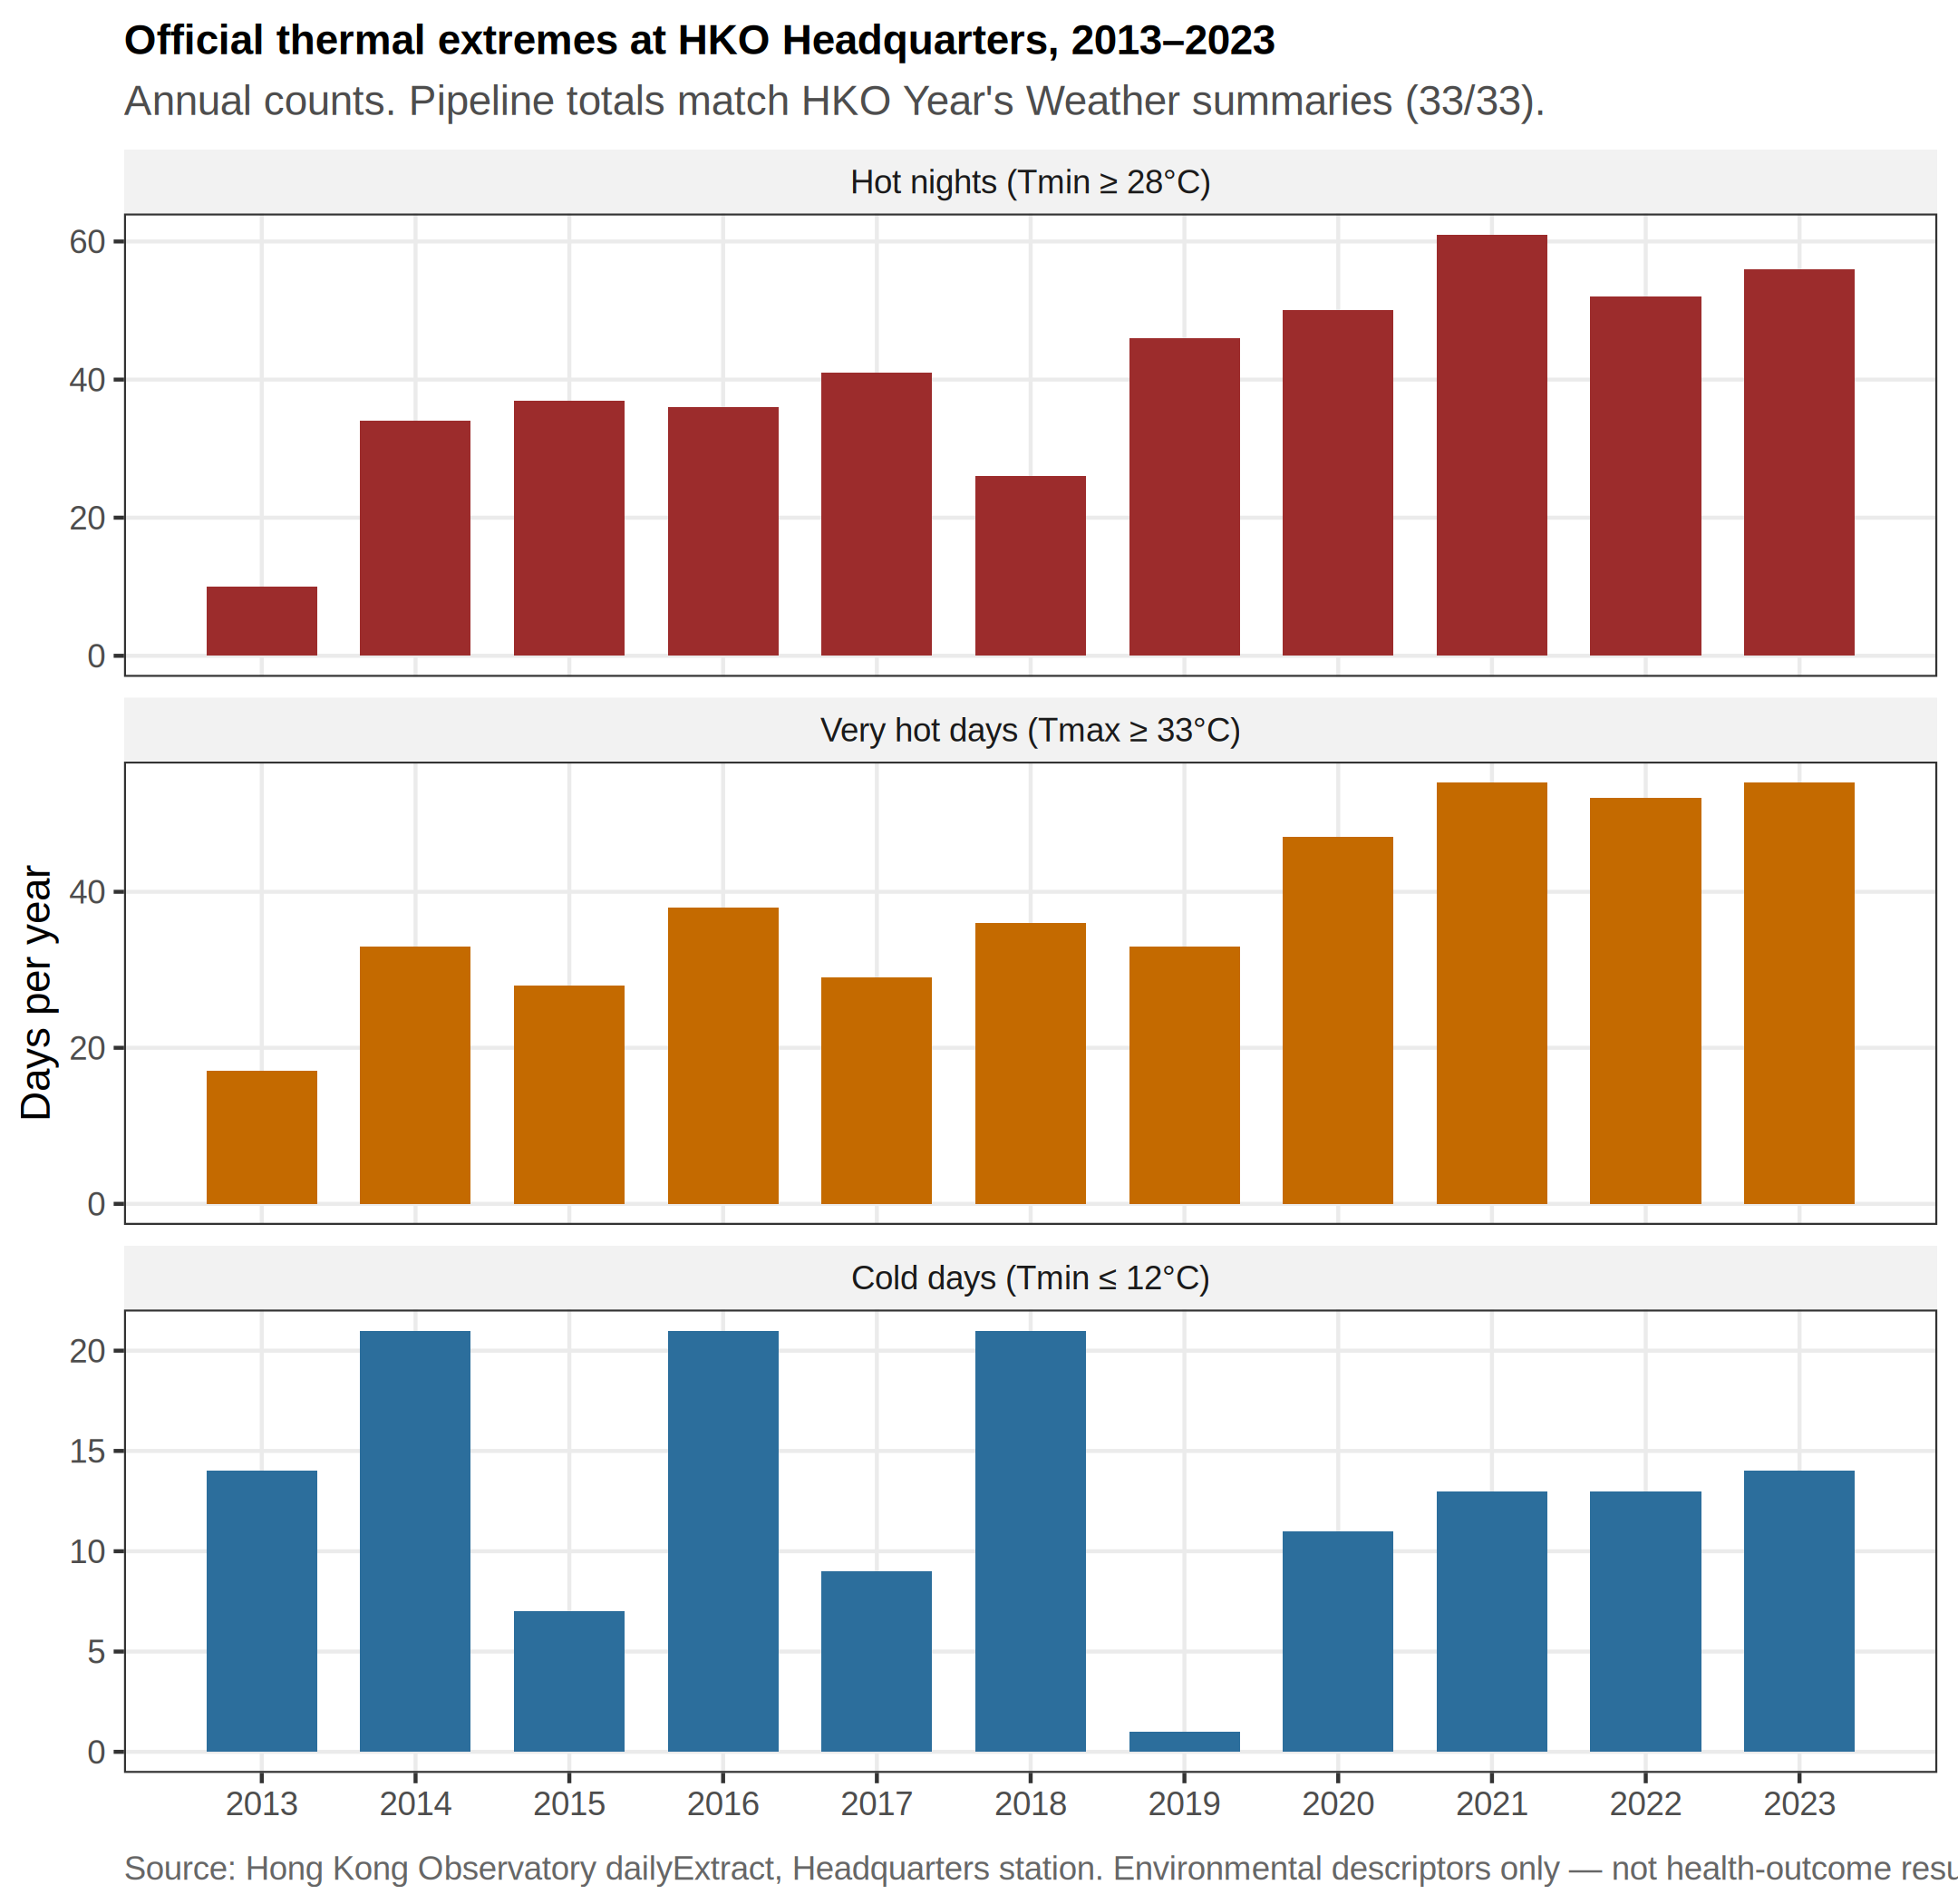
\includegraphics[width=\linewidth,height=260mm,keepaspectratio]{../../figures/exposure_aging/fig01_annual_extremes_coexistence.png}\\[1pt]
\begin{flushleft}
\captext{Annual counts of official HKO extremes at Headquarters. Environmental
descriptors only --- \textbf{not} health-outcome results. Pipeline totals match
HKO \textit{Year's Weather} summaries 33/33.}
\end{flushleft}
\end{secbox}

\begin{secbox}{4. Monthly hot nights and cold days (REAL)}
\body
\centering
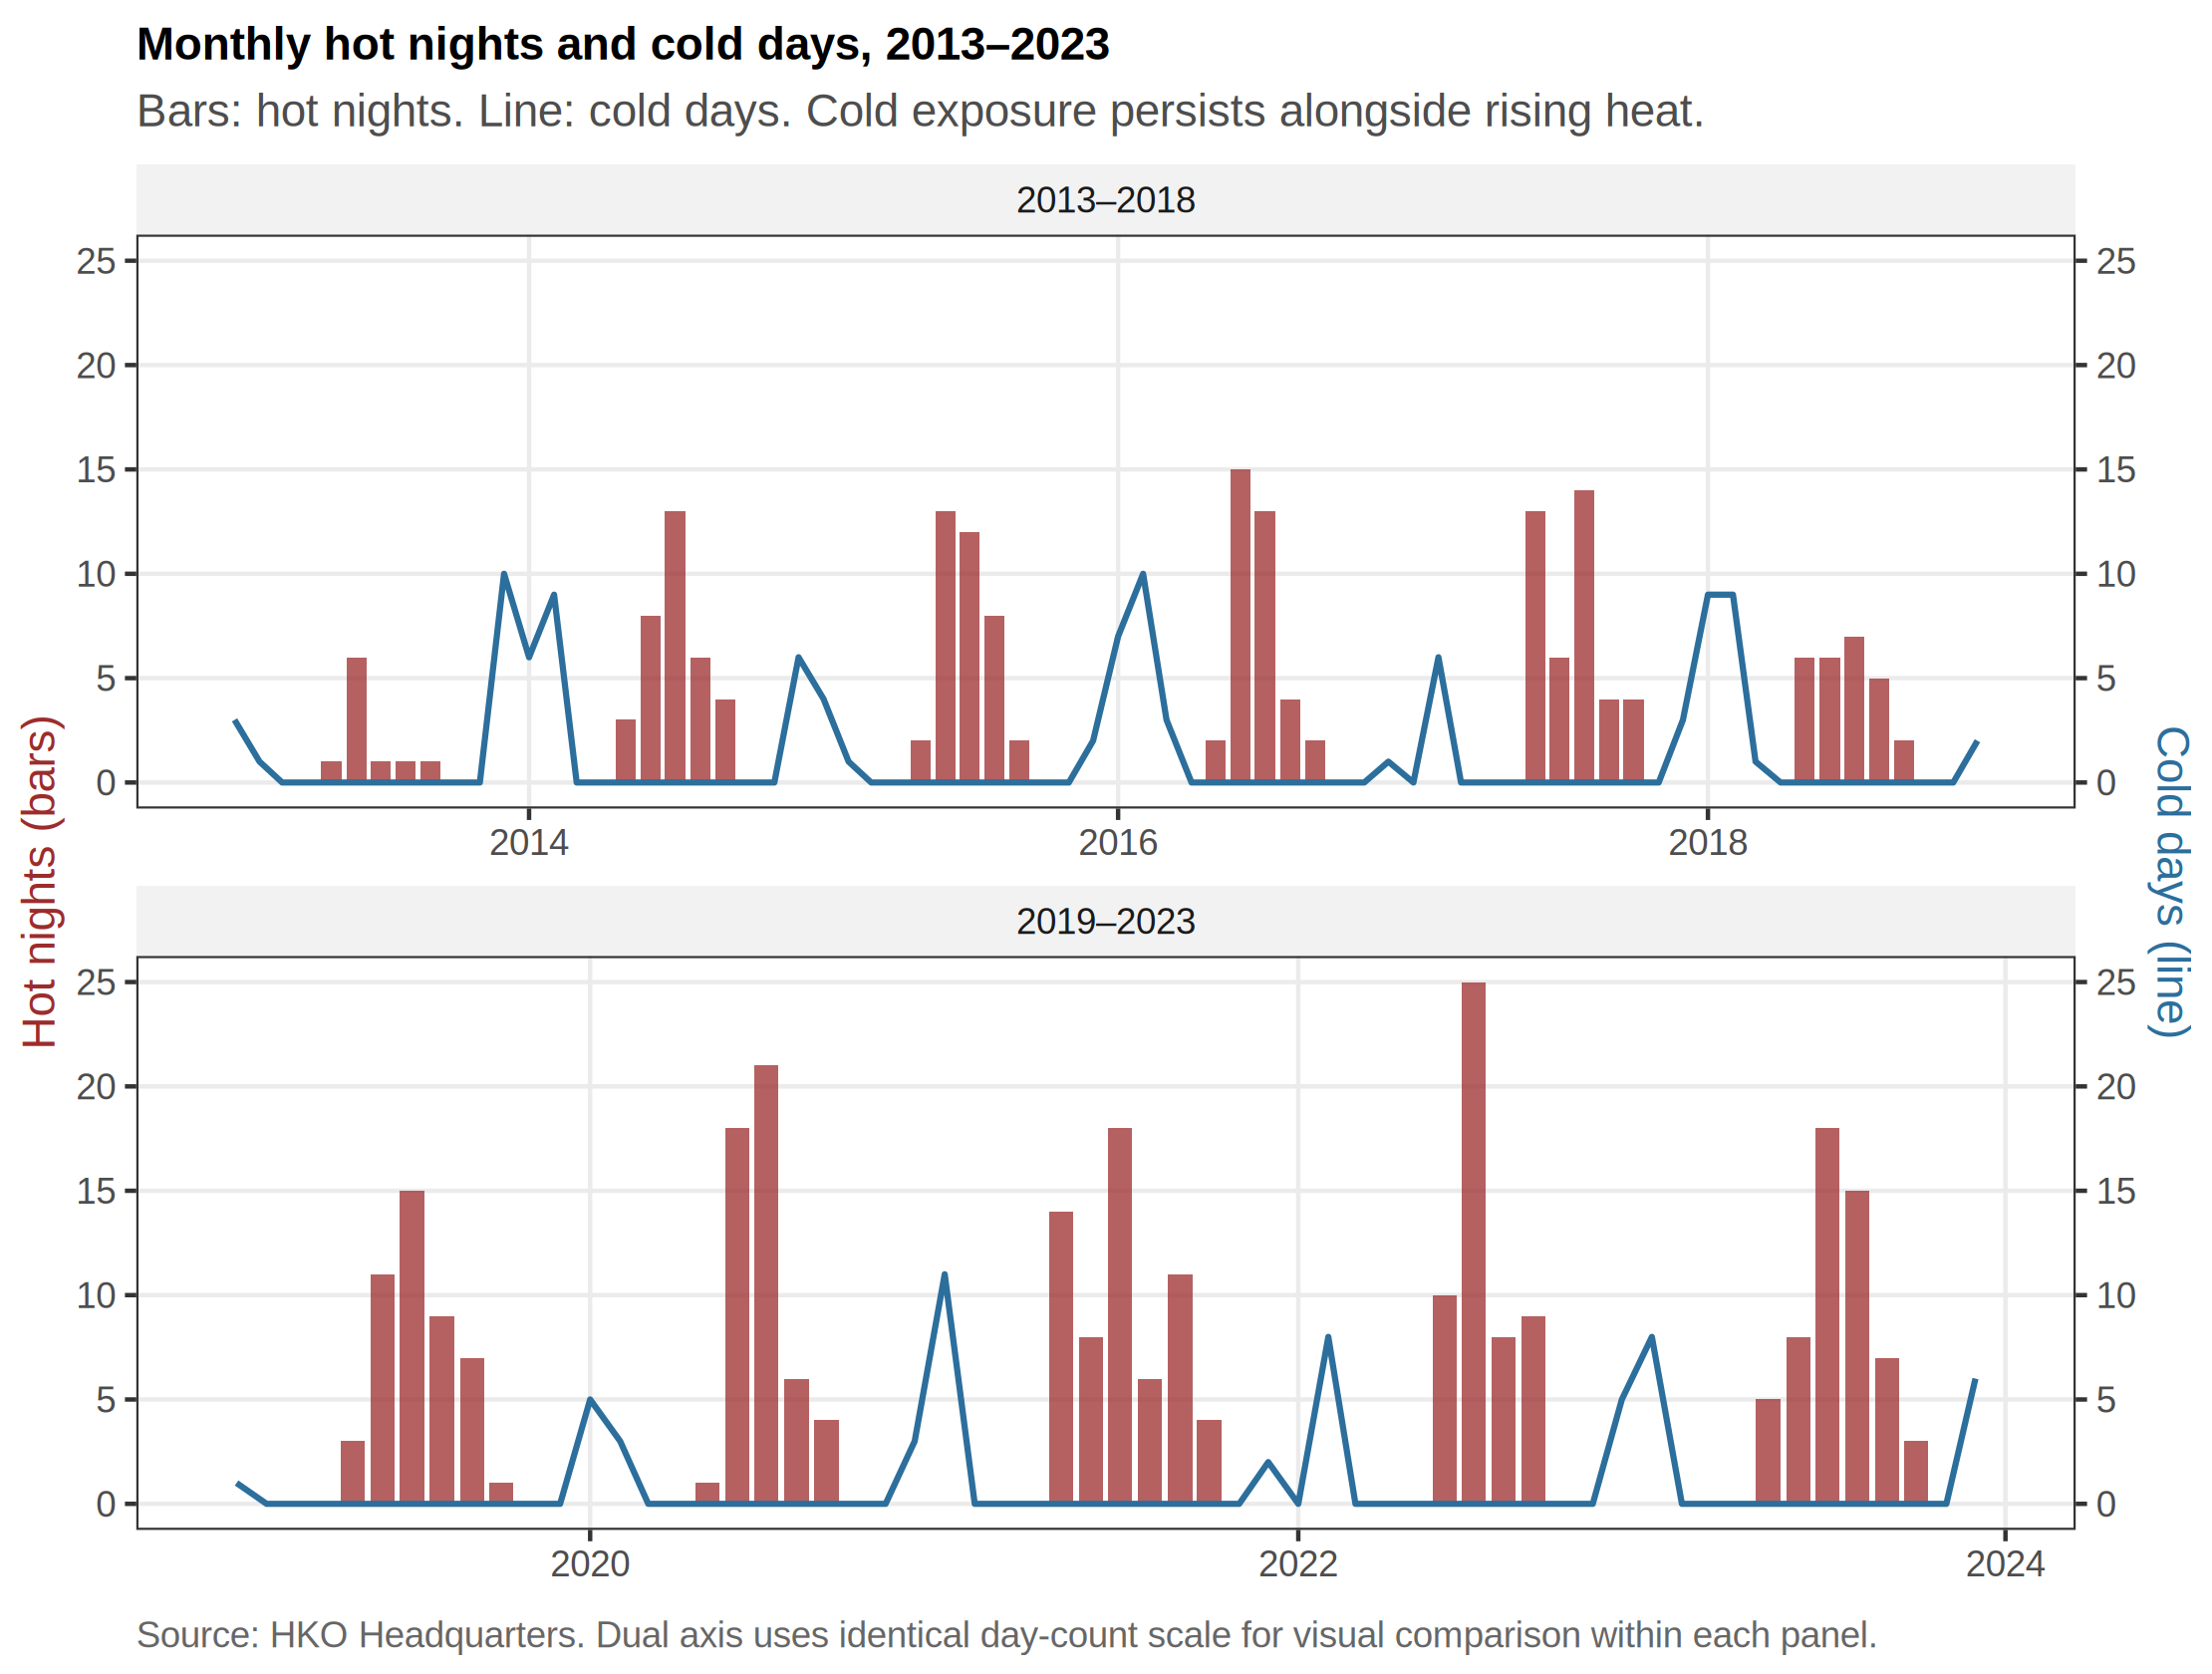
\includegraphics[width=\linewidth,height=212mm,keepaspectratio]{../../figures/exposure_aging/fig02_monthly_hot_nights_cold_days.png}\\[1pt]
\begin{flushleft}
\captext{Monthly official extreme-day counts, 2013--2023: hot nights (bars) climb
while cold days (line) recur every winter. Weather descriptors only.}
\end{flushleft}
\end{secbox}

\begin{secbox}{5. Seasonal pattern of first hospitalisations}
\body
\centering
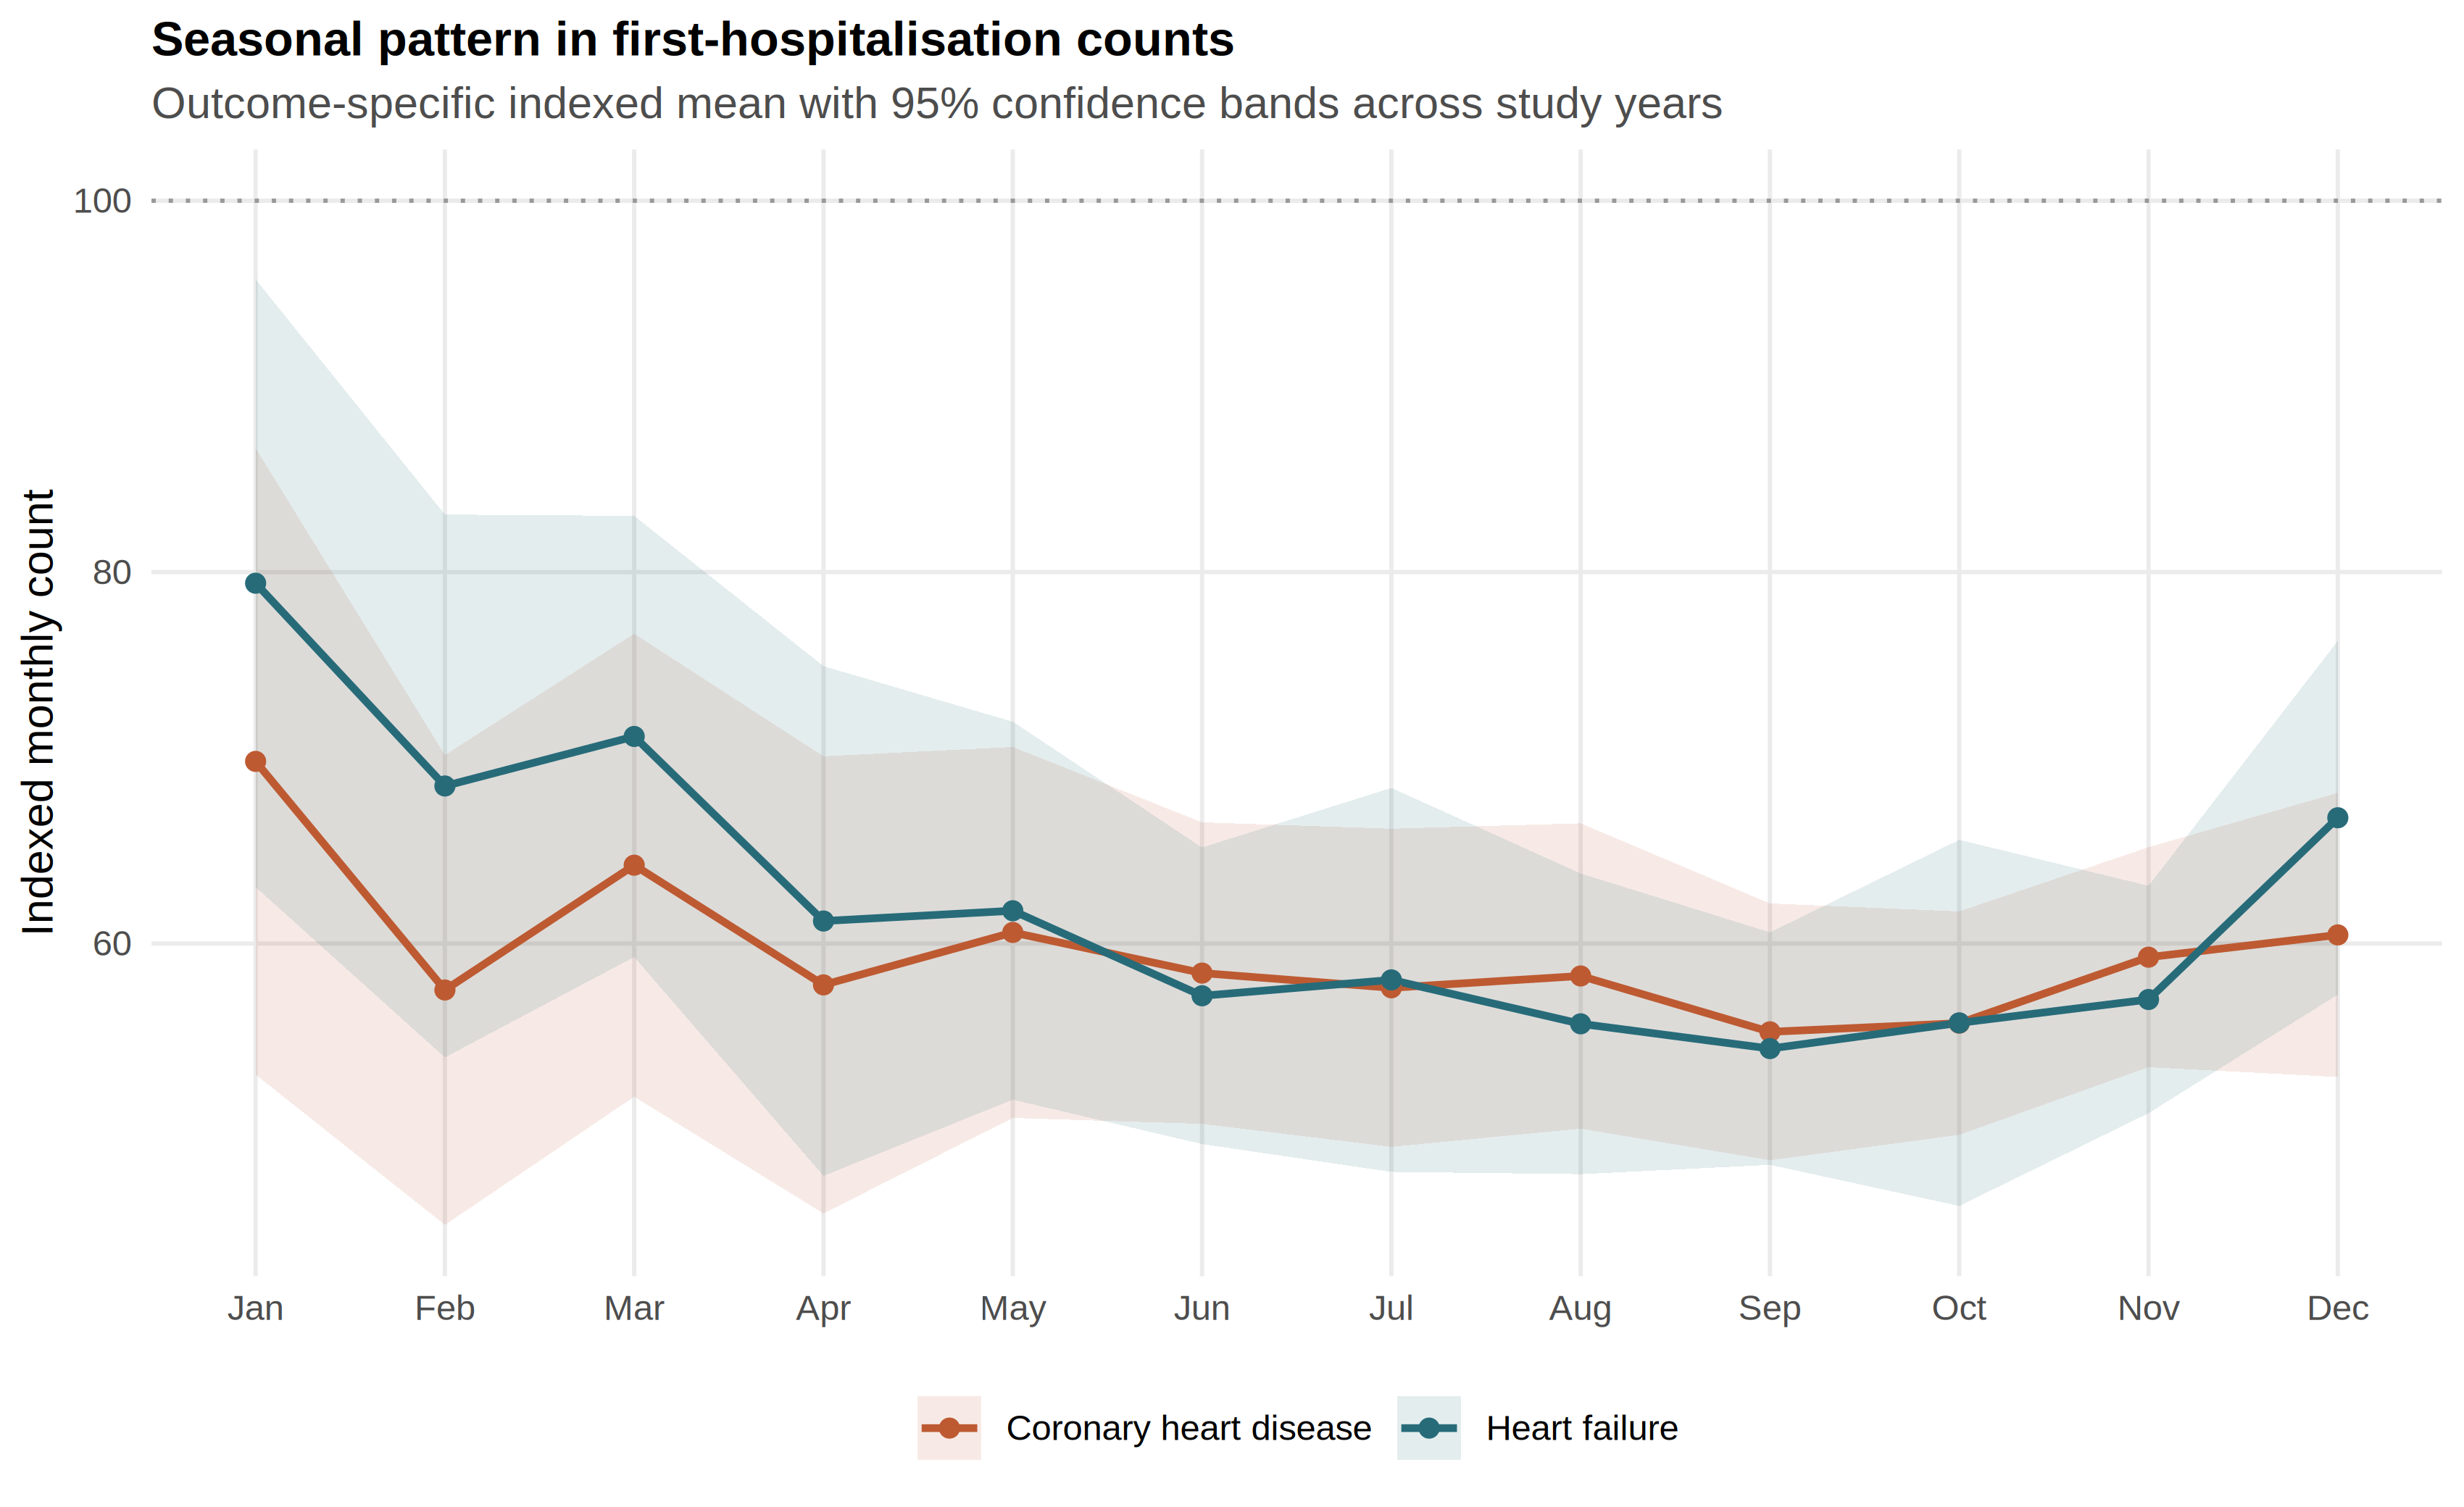
\includegraphics[width=\linewidth,height=226mm,keepaspectratio]{../../outputs/release_chd_hf/figures/figure2_seasonal_pattern.png}\\[1pt]
\begin{flushleft}
\captext{Outcome-specific indexed monthly mean with 95\% bands
(HA\_APPROVED\_AGGREGATE; indexed display --- raw monthly counts are not shown).
Both outcomes peak in winter and trough in early autumn; HF seasonality is the
stronger of the two.}
\end{flushleft}
\end{secbox}

\begin{secbox}[after skip=0pt,height fill,valign=top]{6. Literature map --- estimands are not interchangeable}
\body
{\tbl
\begin{tabularx}{\linewidth}{@{}>{\RaggedRight}p{3.4cm}>{\RaggedRight}X>{\RaggedRight\arraybackslash}p{3.3cm}@{}}
\toprule
\textbf{Study} & \textbf{Quantity} & \textbf{Scale} \\
\midrule
Liu (J.) 2020, \textit{SCS} & CVD \textbf{mortality} attributable fraction; cold fraction $>$ heat fraction & Daily / annual AF \\
Liu (Z.) 2026, medRxiv & Modelled heat-related \textbf{excess deaths} & Daily mortality \\
Goggins 2012/2013 & Cold--stroke / cold--AMI, \% per $^\circ$C cooling & Daily, lagged \\
Guo 2024 & Binary hot-night flag null for excess hospitalisation; night-heat \emph{intensity} informative & Daily \\
\textbf{This project} & \textbf{First CHD/HF hospitalisation}, count ratio per 5 extreme days & \textbf{Monthly ecological} \\
\bottomrule
\end{tabularx}}
\vspace{1.2mm}
Prior Hong Kong work quantifies \emph{mortality} fractions and \emph{daily}
triggering. This project adds the governed \emph{monthly morbidity} layer for
first CHD/HF hospitalisations --- a neighbouring estimand, not a replication.
\begin{warnbox}
{\color{Warn}\smallbody A daily per-$^\circ$C triggering coefficient, a mortality
attributable fraction, and a monthly morbidity count ratio answer different
questions. None may be substituted for another.\par}
\end{warnbox}
\end{secbox}

\end{shell}
\end{minipage}\hfill\begin{minipage}[t]{0.488\textwidth}
% ============================ RIGHT COLUMN ==================================
\begin{shell}[height=1111mm]

\begin{secbox}{7. Methods --- one 12-contrast panel}
\body
\begin{itemize}
  \item \textbf{Panel:} 2 outcomes (CHD, HF) $\times$ 6 exposures
        (mean, Tmax, Tmin per 1$^\circ$C; hot nights, cold days, very hot days
        per 5 days) = 12 pre-specified contrasts
  \item \textbf{Exposures} (official HKO definitions): hot night Tmin\,$\geq$\,28$^\circ$C;
        very hot day Tmax\,$\geq$\,33$^\circ$C; cold day Tmin\,$\leq$\,12$^\circ$C
  \item \textbf{SE ladder} per contrast: Model $\rightarrow$ HC1 $\rightarrow$
        NW3 $\rightarrow$ NW6; continuity decisions use \textbf{NW6}, full ladder shown
  \item \textbf{Multiplicity:} Benjamini--Hochberg $q$ across the 12 core contrasts
  \item Reported as one panel --- not twelve independent ``discoveries''
  \item Full pipeline scripted and re-runnable; release package machine-validated
        before any number reached this poster
\end{itemize}
\end{secbox}

\begin{secbox}{8. Key exploratory results (Gate 3 open)}
\body
\noindent\begin{minipage}[t]{0.485\linewidth}
\begin{tile}[width=\linewidth]
{\color{TealDark}\bfseries\fontsize{19}{21}\selectfont 1.022\ (1.002--1.042)}\\[1pt]
{\fontsize{9.8}{11.6}\selectfont CHD $\times$ hot nights per 5 days; NW6 95\% CI; $p\approx0.032$; $q=0.192$\par}
\end{tile}
\end{minipage}\hfill\begin{minipage}[t]{0.485\linewidth}
\begin{tile}[width=\linewidth]
{\color{TealDark}\bfseries\fontsize{19}{21}\selectfont 1.073\ (1.006--1.144)}\\[1pt]
{\fontsize{9.8}{11.6}\selectfont HF $\times$ cold days per 5 days; NW6 95\% CI; $p\approx0.031$; $q=0.192$\par}
\end{tile}
\end{minipage}
\vspace{1mm}
\begin{itemize}
  \item All 12 core Benjamini--Hochberg $q$-values $>0.19$ ---
        \textbf{no contrast survives multiplicity control}
  \item The CHD hot-night interval \emph{includes the null} under Model and HC1
        standard errors --- the signal is \textbf{SE-sensitive}
  \item Provisional direction pattern (CHD--heat nights; HF--cold) is flagged for
        the Gate~3 discussion, not promoted to a finding
\end{itemize}
\begin{warnbox}
{\color{Warn}\smallbody\textbf{These are exploratory signals.} Gate~3 is open; no
confirmatory headline is claimed on this poster or elsewhere.\par}
\end{warnbox}
\end{secbox}

\begin{secbox}{9. The 12-contrast core at a glance (NW6, exploratory)}
\body
{\tbl
\begin{tabularx}{\linewidth}{@{}l>{\RaggedRight}X>{\RaggedRight\arraybackslash}p{5.2cm}@{}}
\toprule
\textbf{Outcome} & \textbf{Exposure} & \textbf{Count ratio (95\% CI)} \\
\midrule
CHD & Hot nights / 5 days & \textbf{1.022 (1.002--1.042)}, $q=0.192$ \\
CHD & Cold days / 5 days & 0.995 (0.949--1.043), near null \\
CHD & Very hot days / 5 days & 0.999 (0.974--1.025), near null \\
CHD & Mean / Tmax / Tmin per $^\circ$C & $\approx$0.993--0.994, near null \\
\midrule
HF & Cold days / 5 days & \textbf{1.073 (1.006--1.144)}, $q=0.192$ \\
HF & Hot nights / 5 days & 1.003 (0.976--1.031), near null \\
HF & Mean Tmin / $^\circ$C & 0.973 (0.947--1.000), borderline \\
HF & Very hot days / 5 days & 0.995 (0.963--1.028), near null \\
\bottomrule
\end{tabularx}}
\vspace{0.8mm}
\captext{Amended single-exposure core; days-only offset; NW lag-6. Values as
validated in the release panel; do not quote as primary without the team freeze.}
\end{secbox}

\begin{secbox}{10. Core single-exposure models (exploratory)}
\body
\centering
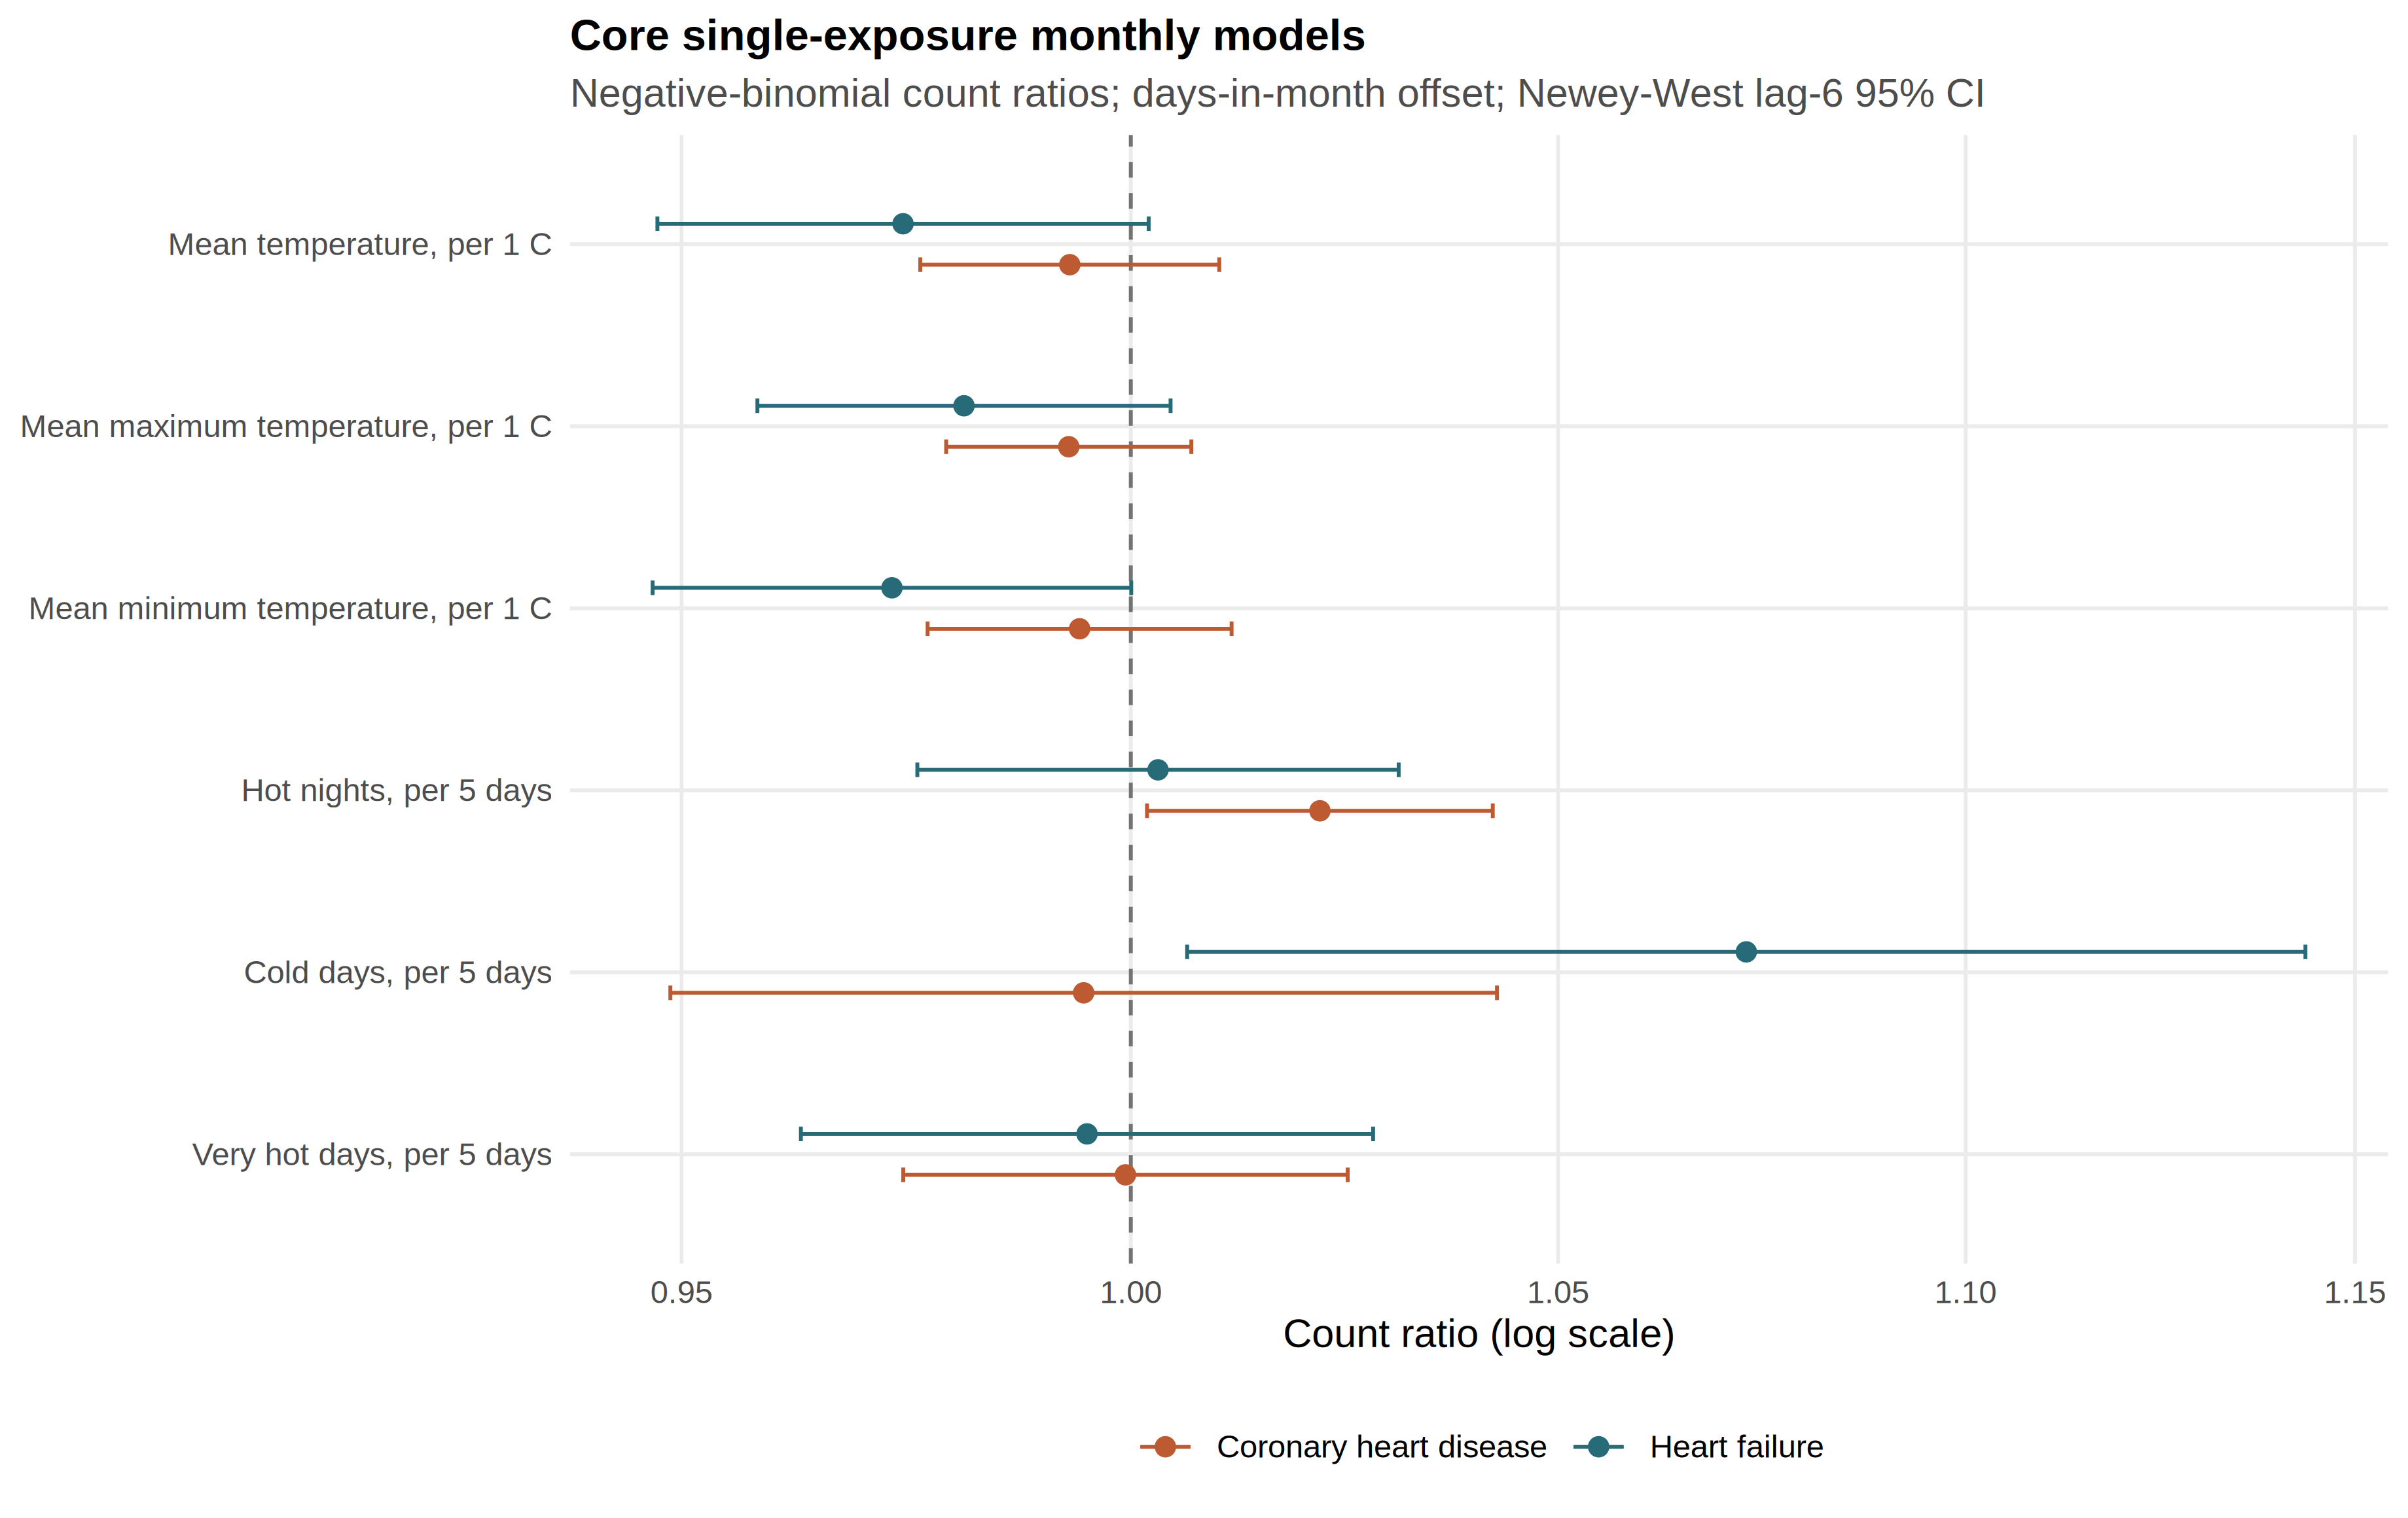
\includegraphics[width=\linewidth,height=243mm,keepaspectratio]{../../outputs/release_chd_hf/figures/figure3_core_forest.png}\\[1pt]
\begin{flushleft}
\captext{Negative-binomial count ratios, days-in-month offset, Newey--West lag-6
95\% intervals. HA\_APPROVED\_AGGREGATE outcomes; Gate~3 open --- exploratory.}
\end{flushleft}
\end{secbox}

\begin{secbox}{11. Uncertainty ladder across SE methods}
\body
\centering
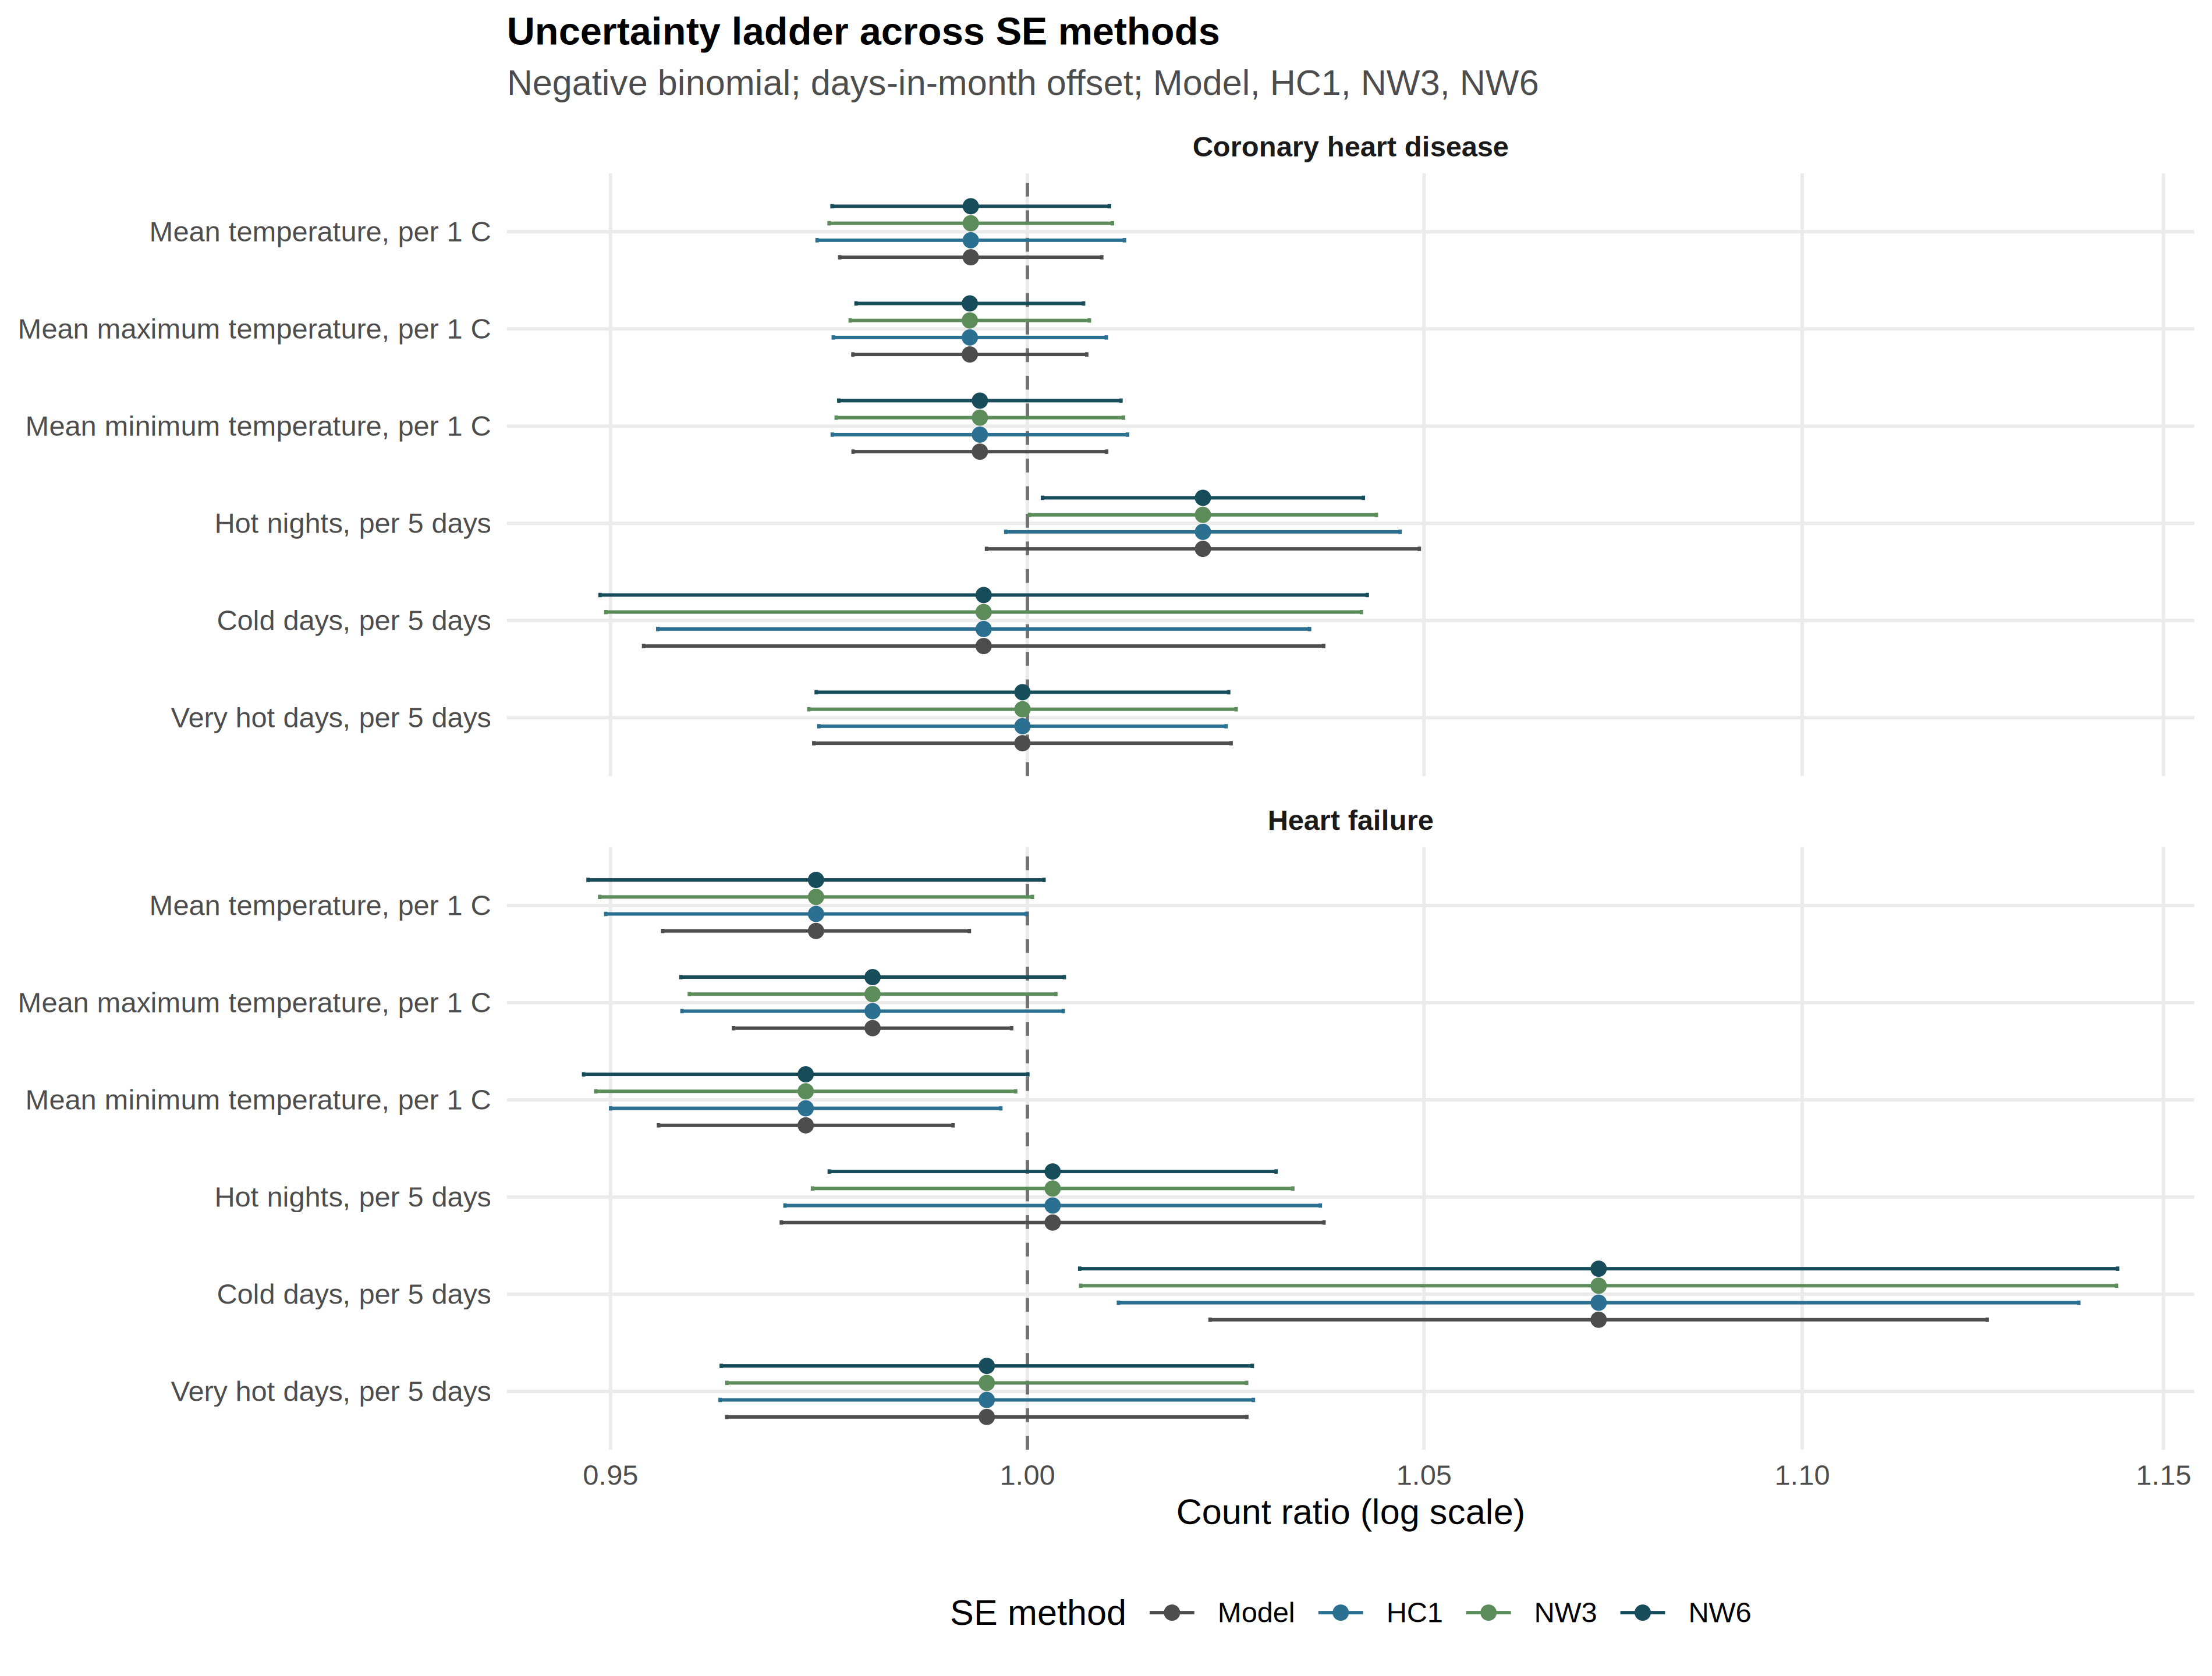
\includegraphics[width=\linewidth,height=292mm,keepaspectratio]{../../outputs/release_chd_hf/figures/figure5_se_method_ladder.png}\\[1pt]
\begin{flushleft}
\captext{The same 12 contrasts under Model, HC1, NW3 and NW6 standard errors.
The HF--cold signal persists across the ladder; the CHD hot-night interval
crosses the null under Model/HC1 --- reported rather than hidden.}
\end{flushleft}
\end{secbox}

\begin{secbox}{12. Feasibility note --- a negative methods result}
\body
A constrained monthly$\to$daily (M\,$|$\,D) downscaling calibration was run under
strict gates (F1.2). It \textbf{failed}: no real daily coefficient was admitted.
This bounds what the method can deliver from monthly aggregates --- a methods
result, \textbf{not} a health finding. The monthly panel remains the resolution
of record.
\end{secbox}

\begin{secbox}{13. Limitations, stated plainly}
\body
\begin{itemize}
  \item Ecological territory-month design --- no individual-level inference
  \item HKO Headquarters is a single-station proxy for territory-wide exposure
  \item Monthly resolution captures \emph{burden}, not day-level triggering
  \item Admission cause unrecorded: outcomes are first hospitalisation
        \emph{after} first CHD/HF diagnosis, not cause-specific events
  \item Multiplicity control limits per-contrast power; near-null intervals do not
        exclude small effects
  \item All estimates provisional until the Gate~3 team freeze
\end{itemize}
\end{secbox}

\begin{secbox}{14. Where to read more}
\body
{\smallbody
\begin{tabularx}{\linewidth}{@{}l>{\RaggedRight\arraybackslash}X@{}}
\toprule
Manuscript & \textsf{manuscript/chd\_hf\_thermal\_associations\_2013\_2023.md} \\
Gate 3 packet & \textsf{reports/gate3\_decision\_packet\_2026-08-07.md} \\
Results panel & \textsf{reports/laidlaw\_stage3/results\_panel\_chd\_hf\_2026-08-07.md} \\
Release & \textsf{outputs/release\_chd\_hf/} (figures, tables, diagnostics) \\
Integrated report & \textsf{reports/bishai\_integrated\_report/} \\
\bottomrule
\end{tabularx}}\\[0.8mm]
Provenance labels used throughout: \textbf{REAL} (HKO, EPD, C\&SD),
\textbf{HA\_APPROVED\_AGGREGATE} (HA outcomes), \textbf{SYNTHETIC} (dev-only;
quarantined, never reported as findings).
\end{secbox}

\begin{secbox}[after skip=0pt,height fill,valign=top]{15. Take-home}
\body
\begin{enumerate}
  \item A reproducible, provenance-labelled monthly panel for CHD/HF
        first-hospitalisation burden now exists end-to-end (132 months;
        REAL weather / population; HA\_APPROVED\_AGGREGATE outcomes;
        release package re-validated).
  \item Two exploratory signals --- CHD with hot nights, HF with cold days ---
        are hypothesis-generating only while Gate~3 remains open.
  \item Honest refusals: no stroke (file not delivered), no principal-diagnosis
        AMI (cause not recorded), no protected primary claim before the team freeze.
  \item Next executable step: the team Gate~3 review of the headline candidates;
        stroke analysis begins only if and when the governed file arrives.
\end{enumerate}
\vspace{1mm}
{\smallbody\textbf{What closes Gate~3:} a team decision freezing (or dropping) the
headline contrast set, with the SE ladder and diagnostics reviewed together.\\[1mm]
\textbf{Contact:} shenrll@connect.hku.hk
\quad\textbar\quad School of Public Health, The University of Hong Kong\par}
\end{secbox}

\end{shell}
\end{minipage}
\vspace{3mm}
% ============================ FOOTER ========================================
\begin{tcolorbox}[enhanced,colback=TealSoft,colframe=Teal,boxrule=0.6pt,arc=0pt,
  left=6pt,right=6pt,top=2.2pt,bottom=2.2pt,before skip=0pt,after skip=0pt,width=\linewidth]
{\fontsize{8.8}{10.6}\selectfont\color{TealDark}
Laidlaw Stage~3 $\cdot$ ISO A0 portrait (841$\times$1189\,mm)
$\cdot$ Collaborators: \textbf{Hogan} (weather definitions \& exposure pipeline)
$\cdot$ \textbf{Zhenyuan Liu / Roro} (Hospital Authority outcome aggregates)
$\cdot$ \textbf{Prof.\ David Bishai} (supervisor)\\[0.4pt]
Provenance: REAL (HKO, EPD, C\&SD) / HA\_APPROVED\_AGGREGATE (HA)
$\cdot$ Gate 3 open --- all health associations exploratory, no confirmatory claim
\hfill shenrll@connect.hku.hk}
\end{tcolorbox}
\end{document}
